\begin{figure}[t]
\centering
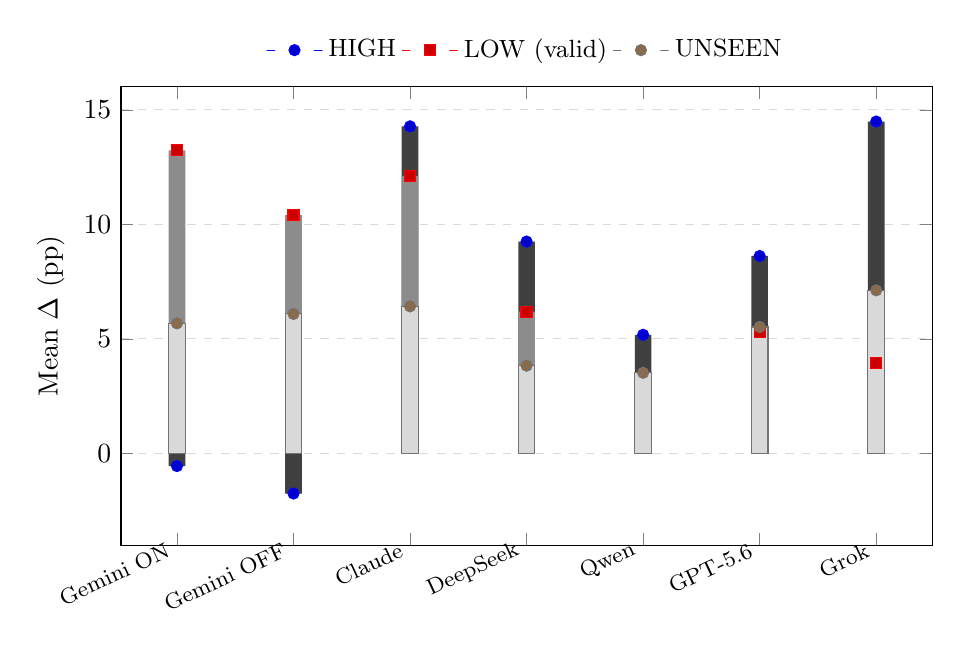
\begin{tikzpicture}
\begin{axis}[
  width=0.98\linewidth,
  height=7.4cm,
  ymajorgrids=true,
  grid style={dashed,gray!30},
  ylabel={Mean $\Delta$ (pp)},
  symbolic x coords={Gemini ON,Gemini OFF,Claude,DeepSeek,Qwen,GPT-5.6,Grok},
  xtick=data,
  x tick label style={rotate=25,anchor=east,font=\footnotesize},
  legend style={at={(0.5,1.03)},anchor=south,legend columns=3,font=\small,draw=none},
  ymin=-4, ymax=16,
  enlarge x limits=0.08,
  bar width=6pt,
]
\addplot+[ybar, fill=black!75, draw=none] coordinates {
  (Gemini ON,-0.55) (Gemini OFF,-1.75) (Claude,14.28) (DeepSeek,9.25)
  (Qwen,5.18) (GPT-5.6,8.62) (Grok,14.49)
};
\addplot+[ybar, fill=black!45, draw=none] coordinates {
  (Gemini ON,13.23) (Gemini OFF,10.40) (Claude,12.11) (DeepSeek,6.19)
  (GPT-5.6,5.31) (Grok,3.95)
};
\addplot+[ybar, fill=black!15, draw=black!55] coordinates {
  (Gemini ON,5.68) (Gemini OFF,6.09) (Claude,6.42) (DeepSeek,3.83)
  (Qwen,3.52) (GPT-5.6,5.52) (Grok,7.12)
};
\legend{HIGH,LOW (valid),UNSEEN}
\end{axis}
\end{tikzpicture}
\caption{Configuration-level mean canonical-coverage $\Delta$ across regimes.
LOW omits Qwen (invalid Direct/Primed model mismatch).
Descriptive only; no inferential intervals.}
\label{fig:configdeltas}
\end{figure}
